\documentclass[../main.tex]{subfiles}

\begin{document}

\subsection{External interfaces requirements}
\subsection{Functional requirements}
	\subsubsection{Use Cases}
	\begin{figure}[htbp]
		\centering
		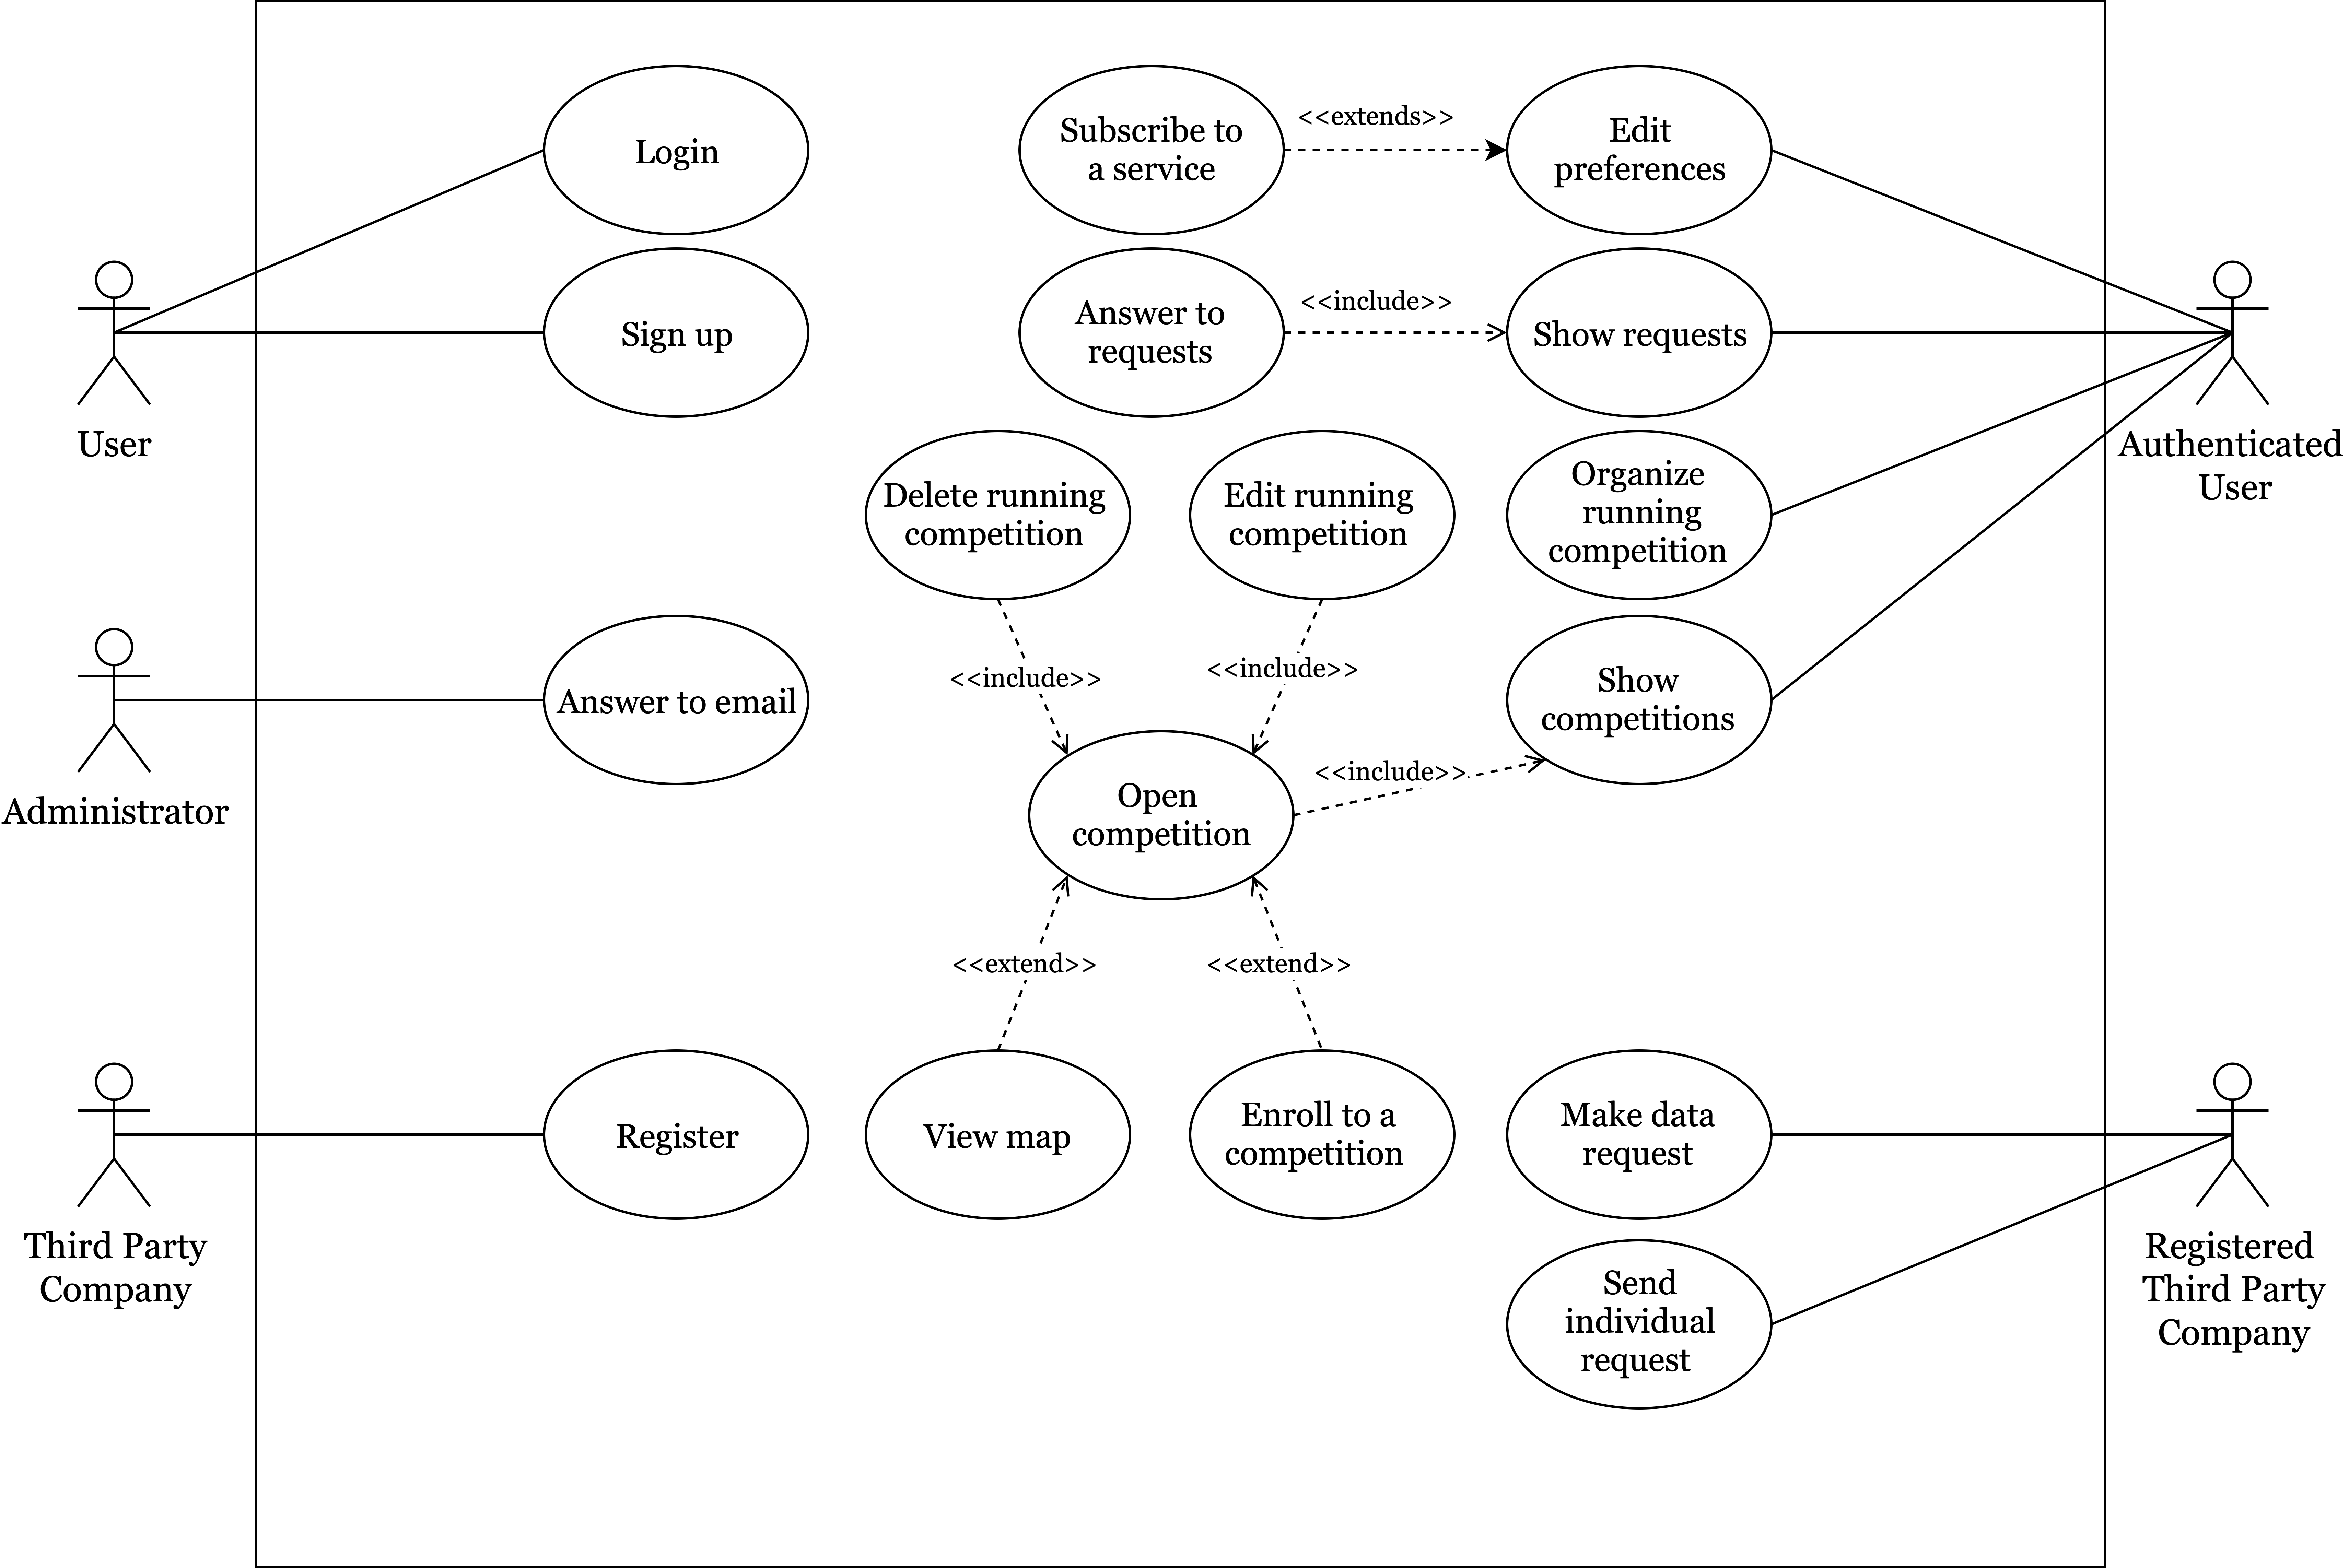
\includegraphics[scale=.052]{img/useCaseTrackMe.png}
		\caption{Use Case Diagram \label{fig:Use Case Diagram}}
	\end{figure}
	\begin{center}
		\begin{tabular}{p{3cm}p{8.28cm}}
			\hline
			\textbf{Use Case} & Sign up\\
			\hline
			\textbf{Actor} & User\\
			\hline
			\textbf{Entry condition} & The user has installed the application on his/her device.\\
			\hline
			\textbf{Flow of events} & \begin{enumerate}
				\linespread{0}\item The user clicks "Sign Up".
				\linespread{0}\item The user fills all mandatory fields.
				\linespread{0}\item The user clicks "Confirm".
			\end{enumerate}\\
			\hline
			\textbf{Exit condition} & The user is registered and now he/she can log in to use the application.\\
			\hline
			\textbf{Exception} & \begin{enumerate}
				\linespread{0}\item The user is already registered.
				\linespread{0}\item The user doesn't fill all mandatory fields.
				\linespread{0}\item The user enters invalid data.
				\linespread{0}\item When an exception occurs the user is notified and the application return to previous page.
			\end{enumerate}\\
			\hline
		\end{tabular}
	\end{center}
	\vspace*{3cm}
	\begin{center}
		\begin{tabular}{p{3cm}p{8.28cm}}
			\hline
			\textbf{Use Case} & Login\\
			\hline
			\textbf{Actor} & User\\
			\hline
			\textbf{Entry condition} & The user has installed the application and it is opened on his/her device.\\
			\hline
			\textbf{Flow of events} & \begin{enumerate}
				\linespread{0}\item The user clicks "Log In".
				\linespread{0}\item The user enters username and password.
				\linespread{0}\item The user decide if he/she wants to be remembered by the system clicking on the relative checkbox.
				\linespread{0}\item The user clicks "Confirm".
				\linespread{0}\item If the user has selected to be remembered, next time the use case ends without asking username and password.
			\end{enumerate}\\
			\hline
			\textbf{Exit condition} & The user is on the home page of the application.\\
			\hline
			\textbf{Exception} & \begin{enumerate}
				\linespread{0}\item The user enters invalid data.
				\linespread{0}\item The user doesn't fill all fields.
				\linespread{0}\item When an exception occurs the user is notified and the application return to previous page.
			\end{enumerate}\\
			\hline
		\end{tabular}
	\end{center}
	\vspace*{3cm}
	\begin{center}
		\begin{tabular}{p{3cm}p{8.28cm}}
			\hline
			\textbf{Use Case} & Register\\
			\hline
			\textbf{Actor} & Third Party Company\\
			\hline
			\textbf{Entry condition} & The third party company is on TrackMe website.\\
			\hline
			\textbf{Flow of events} & \begin{enumerate}
				\linespread{0}\item The third party company go to the registering page.
				\linespread{0}\item The third party company fill all mandatory fields.
				\linespread{0}\item The third party company click on "Send" button. An email with the informations is sent to TrackMe.
			\end{enumerate}\\
			\hline
			\textbf{Exit condition} & The third party company is registered and it's waiting for the Data4Help API key to be received.\\
			\hline
			\textbf{Exception} & \begin{enumerate}
				\linespread{0}\item The third party company enters invalid data.
				\linespread{0}\item The third party company doesn't fill all fields.
				\linespread{0}\item Sending the email fails.
				\linespread{0}\item When an exception occurs the email is not sent and the third party company is notified.
			\end{enumerate}\\
			\hline
		\end{tabular}
	\end{center}
	\vspace*{3cm}
	\begin{center}
		\begin{tabular}{p{3cm}p{8.28cm}}
			\hline
			\textbf{Use Case} & Answer to email\\
			\hline
			\textbf{Actor} & Administrator\\
			\hline
			\textbf{Entry condition} & The administrator has received an email from a third party company.\\
			\hline
			\textbf{Flow of events} & \begin{enumerate}
				\linespread{0}\item The administrator reads the email.
				\linespread{0}\item If the third party company is ok the administrator sends the API key.
				\linespread{0}\item If the third party company isn't ok the administrator sends a rejection email and delete the registration.
			\end{enumerate}\\
			\hline
			\textbf{Exit condition} & The third party company receives the API key and it's ready to use it.\\
			\hline
			\textbf{Exception} & \begin{enumerate}
				\linespread{0}\item Sending the email fails.
				\linespread{0}\item When sending the email fails the administrator is notified.
			\end{enumerate}\\
			\hline
		\end{tabular}
	\end{center}
	\vspace*{3cm}
	\begin{center}
		\begin{tabular}{p{3cm}p{8.28cm}}
			\hline
			\textbf{Use Case} & Edit prefernces\\
			\hline
			\textbf{Actor} & Authenticated User\\
			\hline
			\textbf{Entry condition} & The authenticated user is on the home page of the application.\\
			\hline
			\textbf{Flow of events} & \begin{enumerate}
				\linespread{0}\item The authenticated user selects what service he/she wants to activate: Data4Help, AutomatedSOS, Track4Run.
				\linespread{0}\item The authenticated user can delete the authorization to give data to the third party companies.
				\linespread{0}\item The authenticated user can edit personal informations.
			\end{enumerate}\\
			\hline
			\textbf{Exit condition} & The preferences is saved.\\
			\hline
			\textbf{Exception}\\
			\hline
		\end{tabular}
	\end{center}
	\vspace*{3cm}
	\begin{center}
		\begin{tabular}{p{3cm}p{8.28cm}}
			\hline
			\textbf{Use Case} & Subscribe to a service.\\
			\hline
			\textbf{Actor} & Authenticated User\\
			\hline
			\textbf{Entry condition} & The authenticated user wants to subscribe or unsubscribe to Data4Help, AutomatedSOS and Track4Run.\\
			\hline
			\textbf{Flow of events} & \begin{enumerate}
				\linespread{0}\item The authenticated user opens the preferences.
				\linespread{0}\item The authenticated user clicks a box to subscribe himself to a service.
				\linespread{0}\item If it's required the authenticated user connects his/her wearable device.
			\end{enumerate}\\
			\hline
			\textbf{Exit condition} & The authenticated user is subriscribed to the desired services.\\
			\hline
			\textbf{Exception} & \begin{enumerate}
				\linespread{0}\item The authenticated user doesn't connect the wearable device when requested.
				\linespread{0}\item When an exception occurs the preferences are not saved.
			\end{enumerate}\\
			\hline
		\end{tabular}
	\end{center}
	\vspace*{3cm}
	\begin{center}
		\begin{tabular}{p{3cm}p{8.28cm}}
			\hline
			\textbf{Use Case} & Show requests\\
			\hline
			\textbf{Actor} & Authenticated User\\
			\hline
			\textbf{Entry condition} & The authenticated user is on the home page and wants to see the requests.\\
			\hline
			\textbf{Flow of events} & \begin{enumerate}
				\linespread{0}\item The authenticated user opens the requests page.
				\linespread{0}\item The authenticated user shows the requests.
			\end{enumerate}\\
			\hline
			\textbf{Exit condition} & The requests page is opened and all the requets are visible.\\
			\hline
			\textbf{Exception}\\
			\hline
		\end{tabular}
	\end{center}
	\vspace*{3cm}
	\begin{center}
		\begin{tabular}{p{3cm}p{8.28cm}}
			\hline
			\textbf{Use Case} & Answer to requests\\
			\hline
			\textbf{Actor} & Authenticated User\\
			\hline
			\textbf{Entry condition} & The authenticated user is on the requests page.\\
			\hline
			\textbf{Flow of events} & \begin{enumerate}
				\linespread{0}\item The authenticated user open a request.
				\linespread{0}\item The authenticated user click on "Approve" or "Don't approve".
				\linespread{0}\item When the user approve a data request of a third party company all user's data asked become available to it.
			\end{enumerate}\\
			\hline
			\textbf{Exit condition} & The answers are saved. The requests approved make the relative third party company able to take past data and send new data as soon as available.\\
			\hline
			\textbf{Exception}\\
			\hline
		\end{tabular}
	\end{center}
	\vspace*{3cm}
	\begin{center}
		\begin{tabular}{p{3cm}p{8.28cm}}
			\hline
			\textbf{Use Case} & Organize running competition\\
			\hline
			\textbf{Actor} & Authenticated User\\
			\hline
			\textbf{Entry condition} & The authenticated user is on the home page and wants to organize a running competition.\\
			\hline
			\textbf{Flow of events} & \begin{enumerate}
				\linespread{0}\item The authenticated user clicks "New competition".
				\linespread{0}\item The authenticated user selects the route, date and time.
				\linespread{0}\item The authenticated user clicks "Confirm".
			\end{enumerate}\\
			\hline
			\textbf{Exit condition} & The running competition is organized and now users can show it and enroll to it.\\
			\hline
			\textbf{Exception} & \begin{enumerate}
				\linespread{0}\item There is another running competition in the same place, date and time.
				\linespread{0}\item The route, date or time selected are not valid.
				\linespread{0}\item When an exception occurs the running competition is not saved and the user is notified.
			\end{enumerate}\\
			\hline
		\end{tabular}
	\end{center}
	\vspace*{3cm}
	\begin{center}
		\begin{tabular}{p{3cm}p{8.28cm}}
			\hline
			\textbf{Use Case} & Show competition\\
			\hline
			\textbf{Actor} & Authenticated User\\
			\hline
			\textbf{Entry condition} & The authenticated user is on the home page and wants to show the running competitions.\\
			\hline
			\textbf{Flow of events} & \begin{enumerate}
				\linespread{0}\item The authenticated user clicks "Show competition".
				\linespread{0}\item The authenticated user shows the competitions.
			\end{enumerate}\\
			\hline
			\textbf{Exit condition} & All competitions are visible to user.\\
			\hline
			\textbf{Exception}\\
			\hline
		\end{tabular}
	\end{center}
	\vspace*{3cm}
	\begin{center}
		\begin{tabular}{p{3cm}p{8.28cm}}
			\hline
			\textbf{Use Case} & Open competition\\
			\hline
			\textbf{Actor} & Authenticated User\\
			\hline
			\textbf{Entry condition} & The authenticated user is on the competitions page.\\
			\hline
			\textbf{Flow of events} & \begin{enumerate}
				\linespread{0}\item The authenticated user select a competition.
				\linespread{0}\item The authenticated user shows all details of the competition.
			\end{enumerate}\\
			\hline
			\textbf{Exit condition} & The competition page is opened.\\
			\hline
			\textbf{Exception}\\
			\hline
		\end{tabular}
	\end{center}
	\vspace*{3cm}
	\begin{center}
		\begin{tabular}{p{3cm}p{8.28cm}}
			\hline
			\textbf{Use Case} & Edit run competition\\
			\hline
			\textbf{Actor} & Authenticated User\\
			\hline
			\textbf{Entry condition} & The authenticated user is the creator of the running competition and he/she is on the competition page.\\
			\hline
			\textbf{Flow of events} & \begin{enumerate}
				\linespread{0}\item The authenticated user clicks on "Edit".
				\linespread{0}\item The authenticated user changes route, date and time.
				\linespread{0}\item The authenticated user clicks "Save".
			\end{enumerate}\\
			\hline
			\textbf{Exit condition} & The changes are saved\\
			\hline
			\textbf{Exception}& \begin{enumerate}
				\linespread{0}\item There is another running competition in the same place, date and time.
				\linespread{0}\item The route, date or time selected are not valid.
				\linespread{0}\item When an exception occurs the changes are not saved and the user is notified.
			\end{enumerate}\\
			\hline
		\end{tabular}
	\end{center}
	\vspace*{3cm}
	\begin{center}
		\begin{tabular}{p{3cm}p{8.28cm}}
			\hline
			\textbf{Use Case} & Delete run competition\\
			\hline
			\textbf{Actor} & Authenticated User\\
			\hline
			\textbf{Entry condition} & The authenticated user is the creator of the running competition and he/she is on the competition page.\\
			\hline
			\textbf{Flow of events} & \begin{enumerate}
				\linespread{0}\item The authenticated user clicks on "Delete".
			\end{enumerate}\\
			\hline
			\textbf{Exit condition} & The running competition is deleted and people who were enrolled are notified.\\
			\hline
			\textbf{Exception}& \begin{enumerate}
				\linespread{0}\item The user try to delete a running competition that is in progress.
				\linespread{0}\item When an exception occurs the running competition is not deleted and the user is notified.
			\end{enumerate}\\
			\hline
		\end{tabular}
	\end{center}
	\vspace*{3cm}
	\begin{center}
		\begin{tabular}{p{3cm}p{8.28cm}}
			\hline
			\textbf{Use Case} & Enroll to a competition\\
			\hline
			\textbf{Actor} & Authenticated User\\
			\hline
			\textbf{Entry condition} & The authenticated user is on specific competition page.\\
			\hline
			\textbf{Flow of events} & \begin{enumerate}
				\linespread{0}\item The authenticated user clicks on "Enroll".
			\end{enumerate}\\
			\hline
			\textbf{Exit condition} & The user is enrolled to the competition selected.\\
			\hline
			\textbf{Exception}\\
			\hline
		\end{tabular}
	\end{center}
	\vspace*{3cm}
	\begin{center}
		\begin{tabular}{p{3cm}p{8.28cm}}
			\hline
			\textbf{Use Case} & View map\\
			\hline
			\textbf{Actor} & Authenticated User\\
			\hline
			\textbf{Entry condition} & The authenticated user is on specific competition page.\\
			\hline
			\textbf{Flow of events} & \begin{enumerate}
				\linespread{0}\item The authenticated user clicks on "Map".
			\end{enumerate}\\
			\hline
			\textbf{Exit condition} & The user shows the map of the competition and if it's already start he/she can see the participants location.\\
			\hline
			\textbf{Exception}\\
			\hline
		\end{tabular}
	\end{center}
	\vspace*{3cm}
	\begin{center}
		\begin{tabular}{p{3cm}p{8.28cm}}
			\hline
			\textbf{Use Case} & Make data request\\
			\hline
			\textbf{Actor} & Registered Third party company\\
			\hline
			\textbf{Entry condition} & Third party company has already received the API key.\\
			\hline
			\textbf{Flow of events} & \begin{enumerate}
				\linespread{0}\item Registered third party company makes an html request with some parameters.
			\end{enumerate}\\
			\hline
			\textbf{Exit condition} & Registered third party company received the requested data.\\
			\hline
			\textbf{Exception} & \begin{enumerate}
				\linespread{0}\item Some parameters are not valid.
				\linespread{0}\item The request is rejected because it concerns more than a thousand people. 
				\linespread{0}\item When an error occurs third party company is notified and it doesn't receive requested data. 
			\end{enumerate}\\
			\hline
		\end{tabular}
	\end{center}
	\vspace*{3cm}
	\begin{center}
		\begin{tabular}{p{3cm}p{8.28cm}}
			\hline
			\textbf{Use Case} & Send individual request\\
			\hline
			\textbf{Actor} & Registered Third party company\\
			\hline
			\textbf{Entry condition} & Third party company has already received the API key and it knows fiscal code of the person to whom it's asking for data.\\
			\hline
			\textbf{Flow of events} & \begin{enumerate}
				\linespread{0}\item Registered third party company make an html request with some patameters and the fiscal code of the person.
			\end{enumerate}\\
			\hline
			\textbf{Exit condition} & The request was sent.\\
			\hline
			\textbf{Exception} & \begin{enumerate}
				\linespread{0}\item Some parameters or the fiscal code are not valid.
				\linespread{0}\item When an error occurs third party company is notified and the request is not sent.
			\end{enumerate}\\
			\hline
		\end{tabular}
	\end{center}
\subsection{Performance requirements}
\subsection{Design constraints}
\subsection{Software system attributes}

\end{document}